\documentclass{beamer}

\usepackage[utf8]{inputenc}
\usepackage{subfigure}
\usepackage{bbm}

\usetheme{Madrid}
\usecolortheme{beaver}

\title{Spectral clustering}
\author{%
  Davide Riva
  (\texttt{driva95@protonmail.com})
}

\begin{document}

\frame{\titlepage}

\begin{frame}
  \frametitle{Table of Contents}
  \tableofcontents
\end{frame}

\section{Graphs with 1 connected component}
\begin{frame}
  \frametitle{Graphs with 1 connected component}
  \centering
  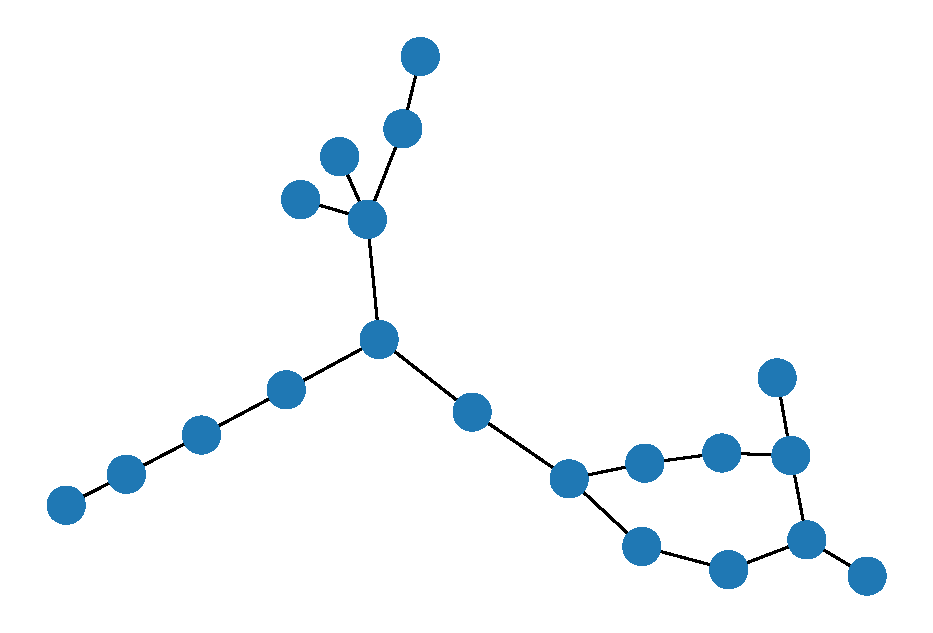
\includegraphics[width=0.5\linewidth]{figures/one-component.eps}
\end{frame}
\begin{frame}
  \begin{block}{Laplacian matrix}
    \[ L = D - W \]
    \[ D_{ij} = \begin{cases} \sum_{j=1}^n W_{ij} \; \text{if} \; i = j \\ 0 \; \text{if} \; i \neq j \end{cases} \]
  \end{block}

  \begin{alertblock}{One eigenvalue equals to zero, its eigenvector equals to $a [1, 1, \dots, 1]$}
    \[ f^T L f = \frac{1}{2} \sum_{i=1}^n \sum_{j=1}^n W_{ij} (f_i - f_j)^2, \; f \in \mathit{R}^n
      \implies f^T L f \geq 0 \; \forall f \]
  \end{alertblock}
\end{frame}

\section{Graphs with multiple connected components}
\begin{frame}
  \frametitle{Graphs with multiple connected components}
  \centering
  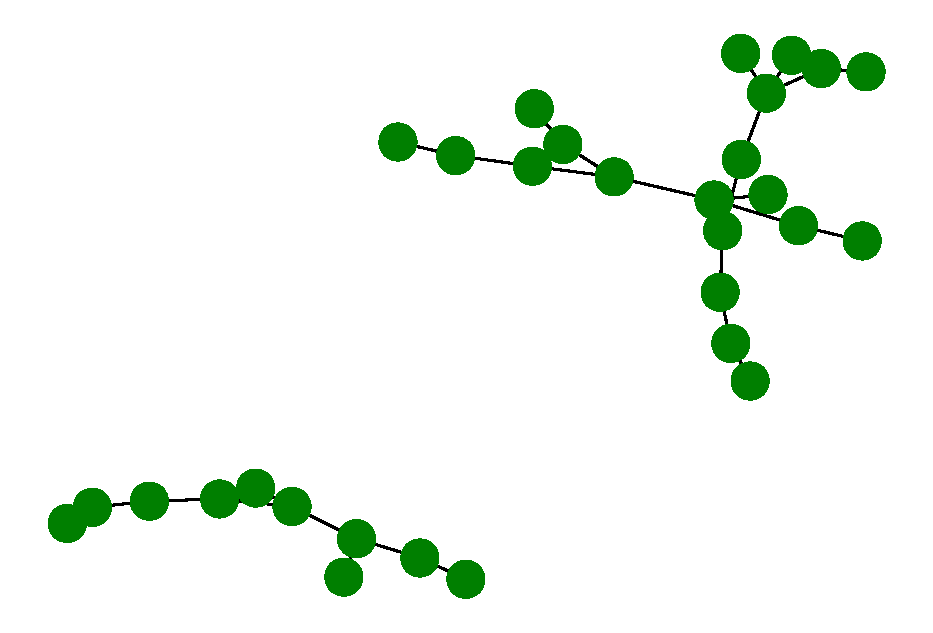
\includegraphics[width=0.5\linewidth]{figures/multiple-component.eps}
\end{frame}

\begin{frame}
  \frametitle{Number of eigenvalues equal to zero}
  \begin{figure}
    \hfill
    \subfigure[Graphs with two connected components]{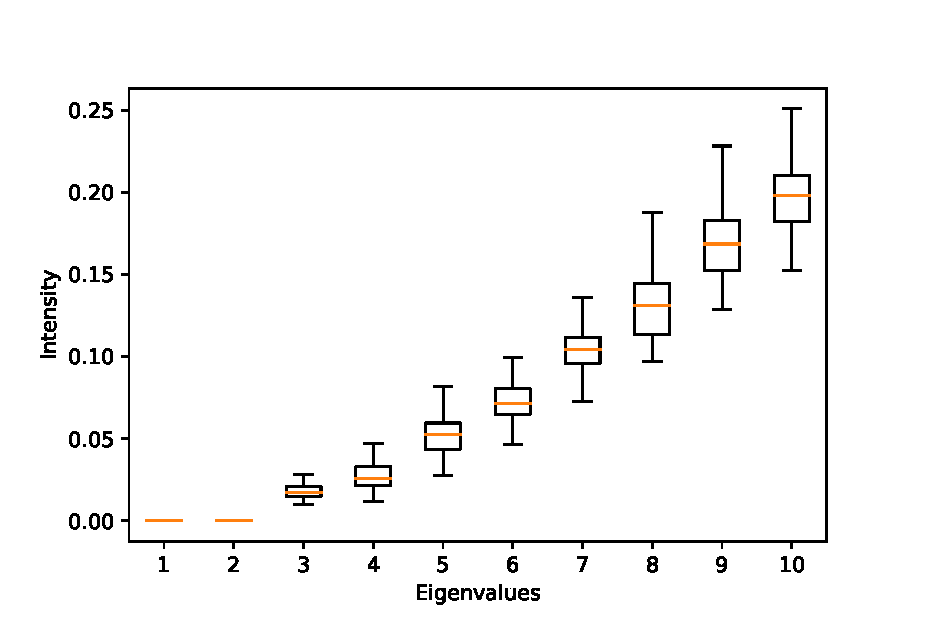
\includegraphics[width=0.3\linewidth]{figures/2-components.eps}}
    \hfill
    \subfigure[Graphs with four connected components]{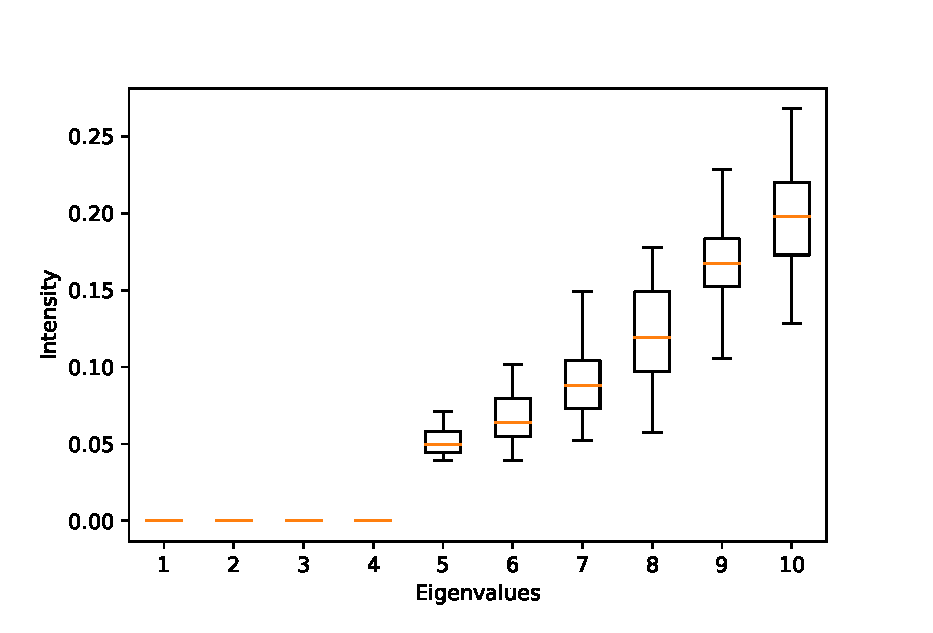
\includegraphics[width=0.3\linewidth]{figures/4-components.eps}}
    \hfill
    \subfigure[Graphs with eight connected components]{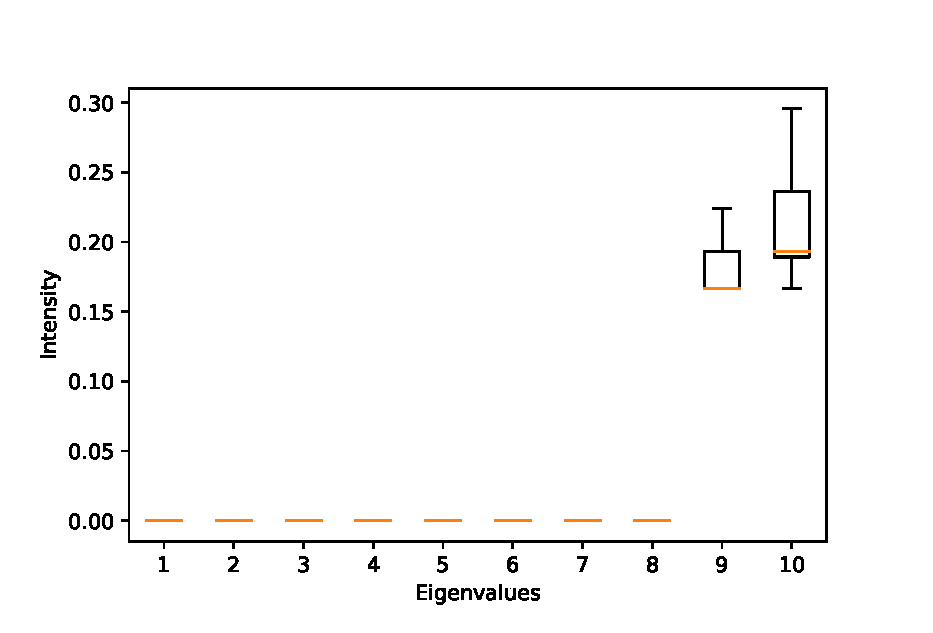
\includegraphics[width=0.3\linewidth]{figures/8-components.eps}}
    \hfill
    \label{figure:mcomp}
    \caption{Box plot of the first 10 eigenvalues of 100 graphs with 64 nodes and different connected components, sorted in ascending order for each graph.}
  \end{figure}
\end{frame}

\begin{frame}
  \frametitle{Eigenvectors as indicator vectors}
  \begin{figure}
    \hfill
    \subfigure{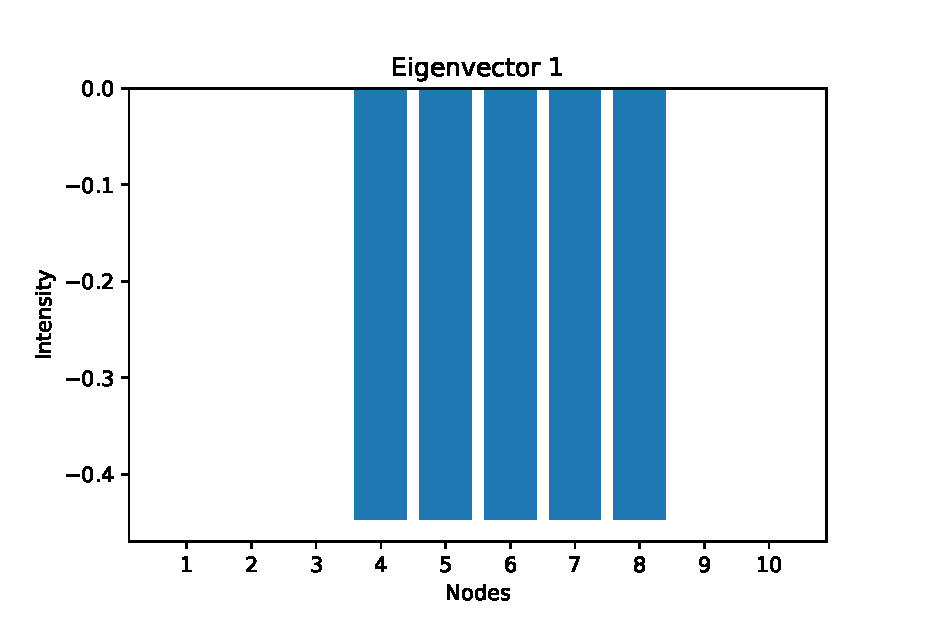
\includegraphics[width=0.3\linewidth]{figures/0-eigenvectors.eps}}%
    \hfill
    \subfigure{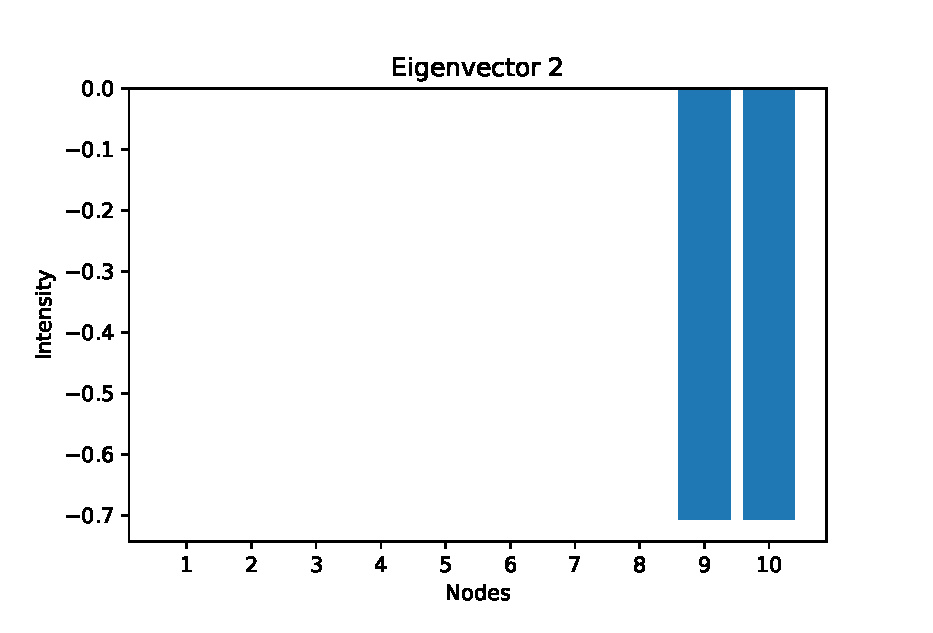
\includegraphics[width=0.3\linewidth]{figures/1-eigenvectors.eps}}%
    \hfill
    \subfigure{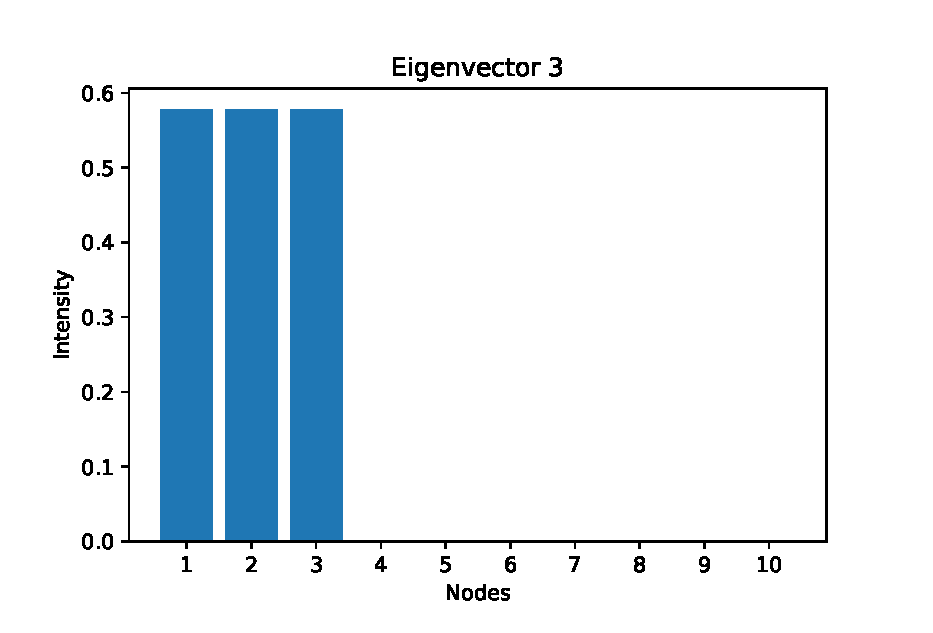
\includegraphics[width=0.3\linewidth]{figures/2-eigenvectors.eps}}%
    \hfill
    \label{figure:eivects}%
  \end{figure}
\end{frame}

\section{Considerations about noise}
\begin{frame}
  \frametitle{Considerations about noise}
  \begin{figure}
    \centering
    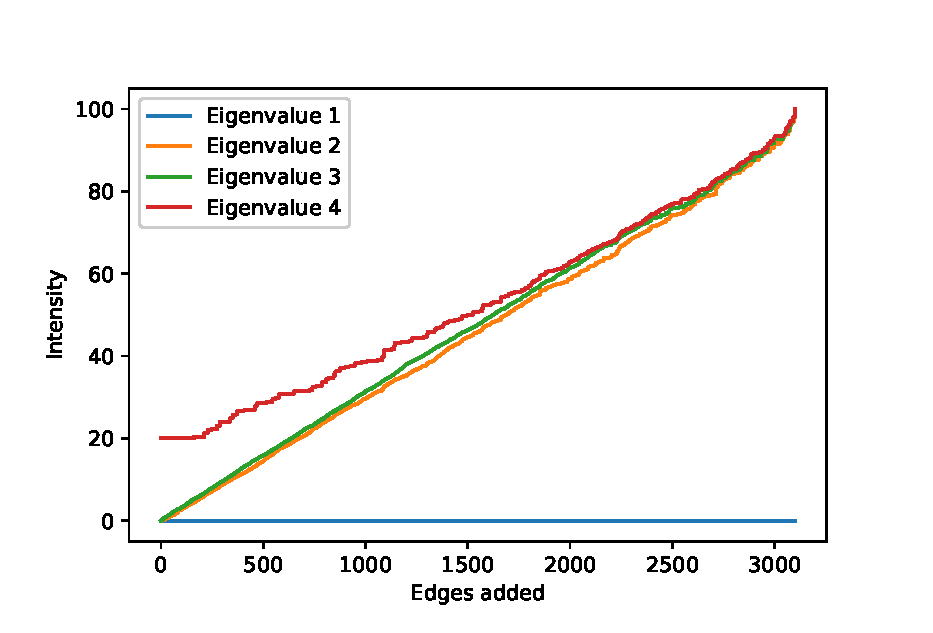
\includegraphics[width=0.5\linewidth]{figures/adding-noise.eps}
    \caption{Example of the effect of noise in the eigenvalues intensities in a graph with 3 connected components}
    \label{figure:addingnoise}
  \end{figure}
\end{frame}

\section{Spectral clustering when data is not a graph}
\begin{frame}
  \frametitle{Spectral clustering when data is not a graph}
  Similarity function $s(x_i, x_j) \geq 0$:
  \begin{itemize}
    \item $s(x_i, x_j) = e^{ - \frac{||x_i - x_j||^2}{2\sigma^2}}$ (Gaussian similarity function)
    \item $s(x_i, x_j) = ||x_i - x_j||_2 < \epsilon$
    \item $s(x_i, x_j) = \frac{1}{\sqrt{2}} \sqrt{\sum_k (\sqrt{x_i(k)} - \sqrt{x_j(k)})^2}$ (Hellinger distance)
    \item \dots
  \end{itemize}
\end{frame}

\begin{frame}
  \frametitle{Why not K-means?}
  \begin{figure}[ht]
    \hfill
    \subfigure[Ground truth]{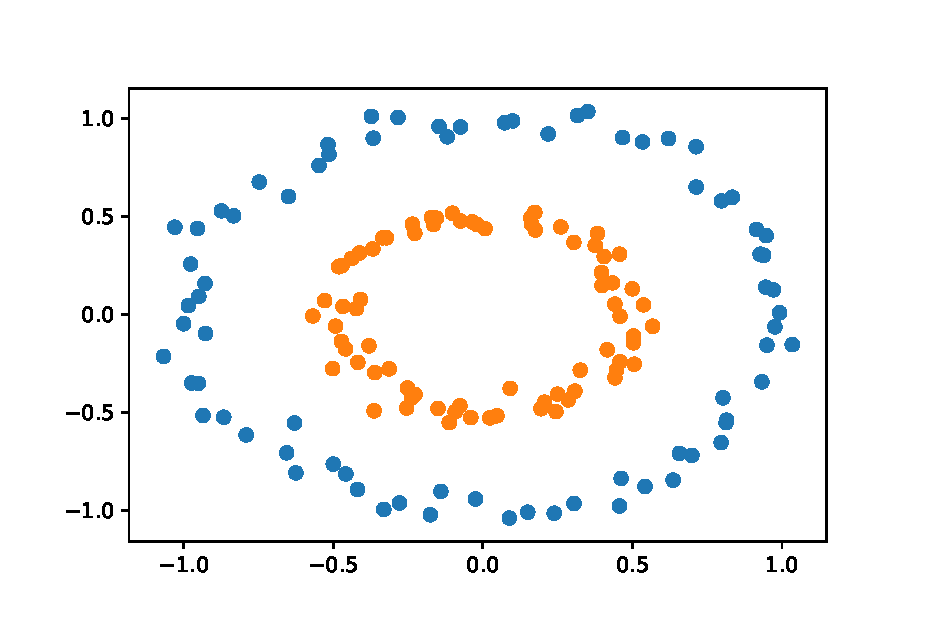
\includegraphics[width=0.3\linewidth]{figures/ground-truth.eps}}%
    \hfill
    \subfigure[Clustering using K-means]{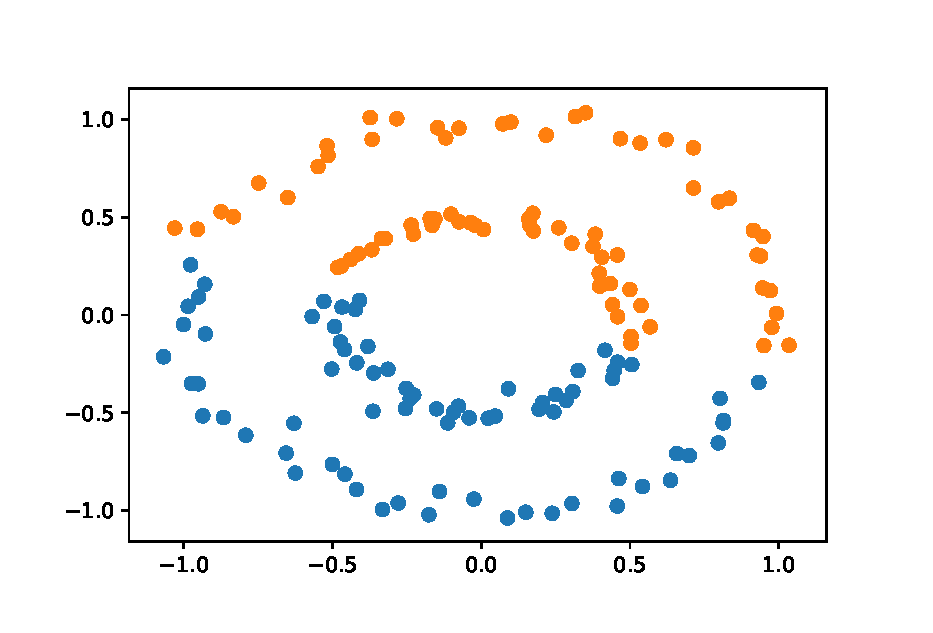
\includegraphics[width=0.3\linewidth]{figures/kmeans.eps}}%
    \hfill
    \subfigure[Clustering using spectral clustering]{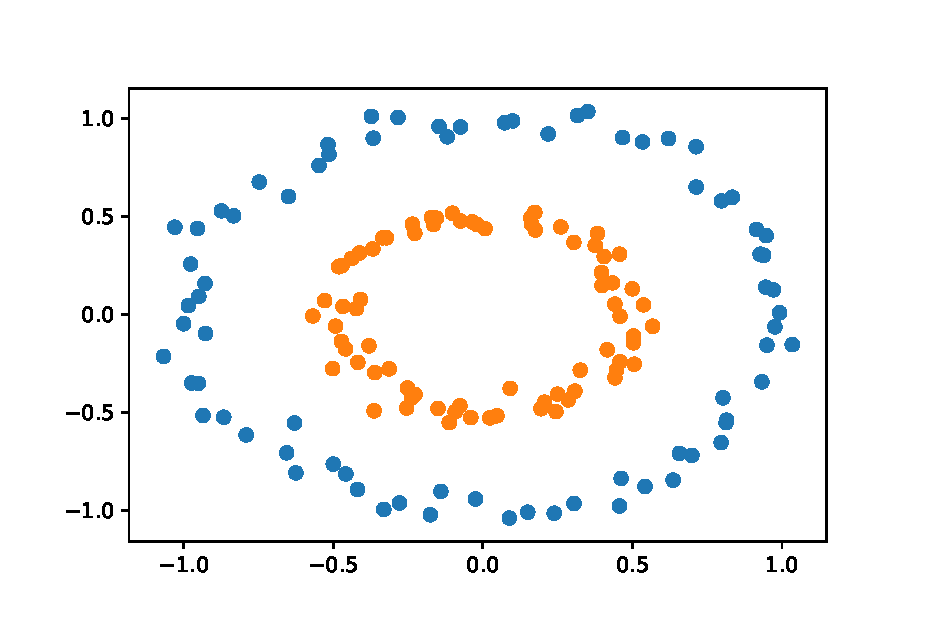
\includegraphics[width=0.3\linewidth]{figures/spectral-on-comparison.eps}}%

  \end{figure}
\end{frame}

\begin{frame}
  \frametitle{Is it possible to avoid hyperparameters tuning?}
  \begin{block}{Modularity}
    \[ Q = \frac{1}{2m} \sum_{i=1}^n \sum_{j=1}^n (A_{ij} - \frac{k_i k_j}{2m}) \mathbbm{1}_{[C_i == C_j]} \]
  \end{block}

  \begin{figure}
    \subfigure[Raw data]{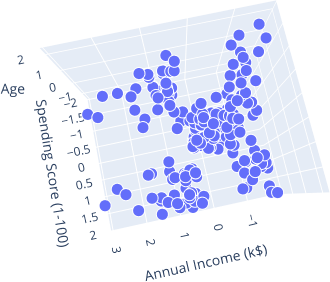
\includegraphics[width=0.2\linewidth]{figures/mall-raw.png}}%
    \hfill
    \subfigure[Spectral clustering with modularity]{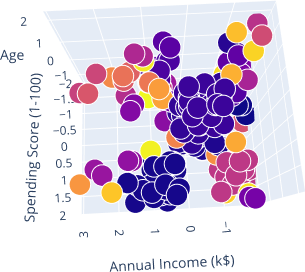
\includegraphics[width=0.2\linewidth]{figures/mall-spectral.png}}%
    \hfill
    \subfigure[Spectral clustering]{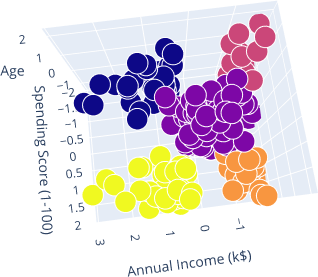
\includegraphics[width=0.2\linewidth]{figures/mall-manual.png}}%
  \end{figure}
\end{frame}

\begin{frame}
  \frametitle{Conclusions}
  Spectral clustering outperforms K-means, but you need hyperparameter tuning
\end{frame}

\end{document}